\documentclass[a4paper, 12pt]{ctexart}

\usepackage{geometry}
\geometry{left=2.5cm, right=2.5cm, top=3cm, bottom=3cm}
\usepackage{graphicx}
\usepackage{booktabs}
\usepackage{tabularx}
\usepackage{multirow}
\usepackage{makecell}
\usepackage{float}
\usepackage{xcolor}
\usepackage{listings}
\usepackage[hidelinks]{hyperref}
\usepackage{amsmath}
\usepackage{caption}
\usepackage{subcaption}
\usepackage{tikz}
\usetikzlibrary{arrows.meta, positioning, shapes.geometric}

\emergencystretch=3em
\graphicspath{{images/}}

\lstset{
    basicstyle=\ttfamily\footnotesize,
    keywordstyle=\color{blue!70!black}\bfseries,
    stringstyle=\color{red!70!black},
    commentstyle=\color{green!45!black}\itshape,
    breaklines=true,
    numbers=left,
    numberstyle=\tiny\color{gray},
    frame=single,
    backgroundcolor=\color{gray!5},
    captionpos=b,
    showstringspaces=false
}

\title{\textbf{鸡尾酒会语音分离实验报告}}
\author{姓名：李好 \quad 学号：22920242203269}
\date{}

\begin{document}

\begin{titlepage}
	\centering
	\vspace*{0.5cm} % 【修改】从 1.2cm 缩小到 0.5cm
	
\includegraphics[width=4.5cm]{Xiamen_University_logo.svg.png}
	\vspace{0.8cm} % 【修改】从 1.3cm 缩小到 0.8cm
	
	{\Huge \textbf{艺术认知与计算}\par}
	\vspace{0.5cm} % 【修改】微调标题间距
	{\Huge \textbf{实验报告}\par}
	\vspace{1.2cm} % 【修改】从 2.0cm 缩小到 1.2cm
	
	{\Large
		\renewcommand{\arraystretch}{1.5} % 【修改】行距从 1.8 缩小到 1.5，这能省下很多空间
		\renewcommand{\arraystretch}{1.5}
		\begin{tabular}{l l}
			\makebox[4em][s]{\textbf{实验题目}}： & \underline{\makebox[9cm][c]{\textbf{鸡尾酒会语音分离实验}}} \\
			\makebox[4em][s]{\textbf{实验内容}}： & \underline{\makebox[9cm][c]{\textbf{双说话人混合语音盲分离}}} \\
			\makebox[4em][s]{\textbf{专业}}： & \underline{\makebox[9cm][c]{\textbf{人工智能}}} \\
			\makebox[4em][s]{\textbf{姓名}}： & \underline{\makebox[9cm][c]{\textbf{李好}}} \\
			\makebox[4em][s]{\textbf{学号}}： & \underline{\makebox[9cm][c]{\textbf{22920242203269}}} \\
			\makebox[4em][s]{\textbf{实验日期}}： & \underline{\makebox[9cm][c]{\textbf{2026年6月}}} \\
			\makebox[4em][s]{\textbf{指导教师}}： & \underline{\makebox[9cm][c]{\textbf{吴梅红}}} \\
		\end{tabular}
		\par}
	
	\vfill
	{\large 本报告基于 LibriSpeech 语音数据、ESC-50 环境噪声、BLSTM 软掩码分离模型以及 Streamlit GUI 展示系统完成。\par}
\end{titlepage}

\newpage
\tableofcontents
\newpage

\section{实验目的}

鸡尾酒会问题描述的是在多人同时说话或存在环境噪声时，从混合声音中恢复目标说话人语音的任务。本实验围绕双说话人单通道语音盲分离展开：输入为一段单通道混合语音，输出为两路尽可能对应原始说话人的分离语音。

本实验的主要目标如下：

\begin{enumerate}
    \item \textbf{完成语音分离完整流程}：从真实语音数据准备、混合语音生成、训练集与验证集划分，到模型训练、语音重建和指标评估，形成可复现实验链路。
    \item \textbf{理解时频域语音分离方法}：使用 STFT 将波形转换到时频域，利用模型预测每个说话人的软掩码，再通过 ISTFT 重建分离后的语音。
    \item \textbf{实现并验证 BLSTM 分离模型}：采用双向 LSTM 提取时序上下文信息，使用软掩码分支预测两路说话人掩码，并以置换不变的信号逼近损失进行训练。
    \item \textbf{设计 Easy 与 Hard 对比实验}：Easy 实验用于验证模型在相对简单场景下的分离能力；Hard 实验加入更多说话人和真实环境噪声，用于考察模型在困难条件下的表现变化。
    \item \textbf{构建 GUI 展示界面}：通过 Streamlit 展示混合语音、参考源、分离结果、波形、频谱和 SI-SDR 指标，使实验结果可以被直观听到和看到。
\end{enumerate}

图 \ref{fig:pipeline} 展示了本实验的整体流程。该流程以 LibriSpeech 纯净语音为输入，通过数据生成脚本合成双说话人混合语音；模型在 STFT 幅度谱特征上训练，输出软掩码并重建语音；最后使用 SI-SDR 与 Delta SDR 评估分离质量。

\begin{figure}[H]
    \centering
    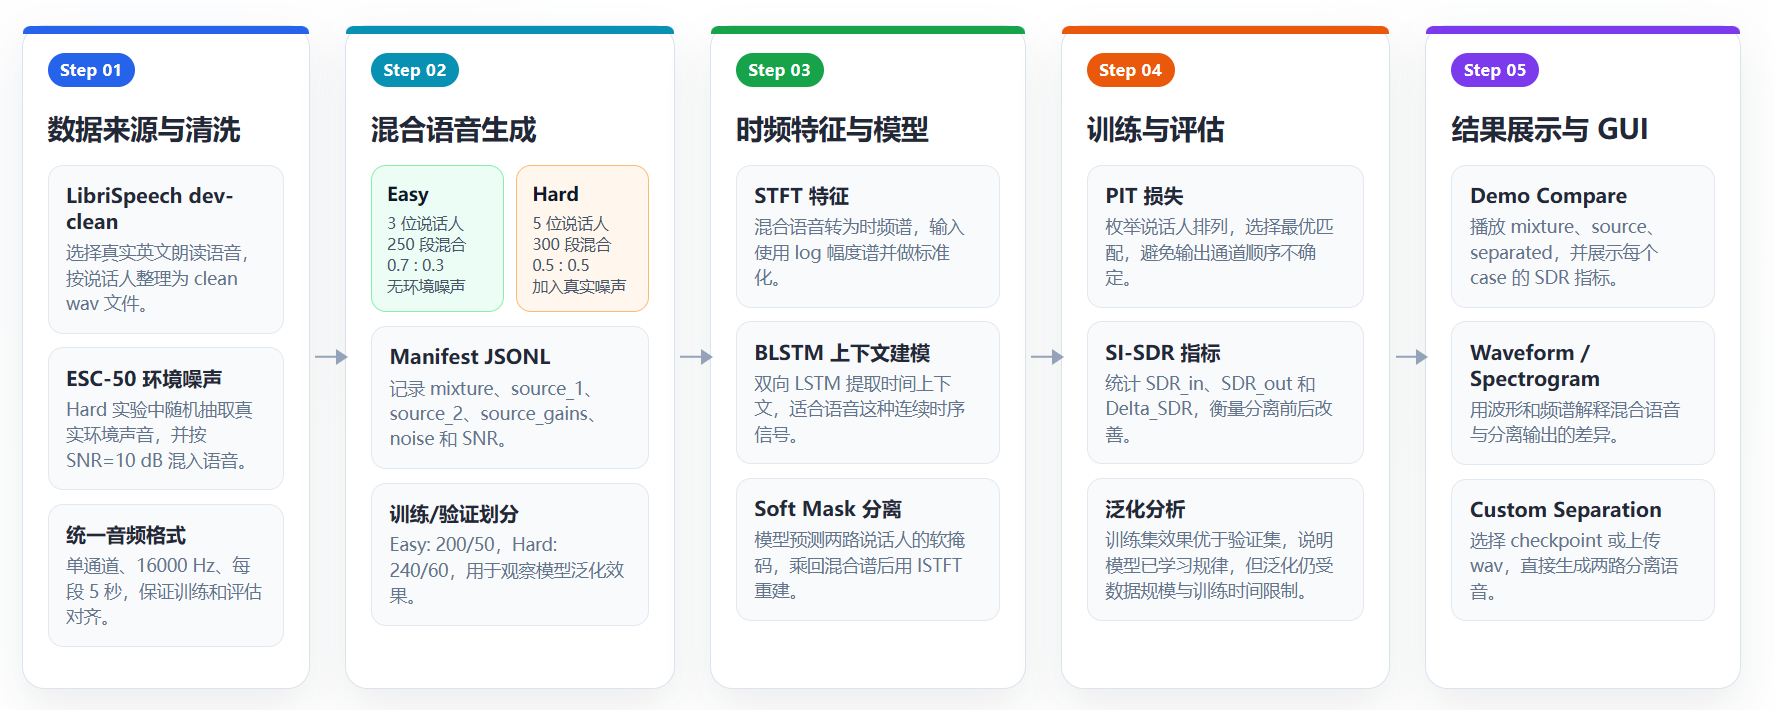
\includegraphics[width=0.95\textwidth]{pipeline_diagram.png}
    \caption{鸡尾酒会语音分离实验流程}
    \label{fig:pipeline}
\end{figure}

\section{数据来源与实验设计}

\subsection{数据来源}

实验语音来源于 LibriSpeech 数据集中的 \texttt{dev-clean} 子集。LibriSpeech 是由有声书语音整理得到的公开英文语音数据集，语音较清晰，适合用于基础语音识别与语音分离实验 \cite{panayotov2015librispeech}。本实验下载文件为：

\begin{center}
\url{https://www.openslr.org/resources/12/dev-clean.tar.gz}
\end{center}

Hard 实验中的真实环境噪声来源于 ESC-50 数据集。ESC-50 包含多类真实环境声音，例如风声、车辆声、动物声、室内外背景声等 \cite{piczak2015esc}。实验中从 ESC-50 的音频目录中随机选择噪声片段，并按指定信噪比混入双说话人语音。

\begin{center}
\url{https://github.com/karolpiczak/ESC-50/archive/refs/heads/master.zip}
\end{center}

\subsection{数据生成流程}

原始 LibriSpeech 文件为 FLAC 格式。实验首先使用 \texttt{prepare\_librispeech\_clean.py} 将选中的说话人语音转换为单通道 WAV 文件，并整理为按说话人划分的文件夹。随后使用 \texttt{build\_dataset\_manifest.py} 随机抽取两个不同说话人的语音片段，裁剪或补零到统一长度，按指定能量比例混合，并生成如下三类文件：

\begin{itemize}
    \item \textbf{mixture}：双说话人混合语音；
    \item \textbf{source}：与混合语音严格对齐的两个参考源贡献；
    \item \textbf{manifest}：记录混合语音路径、参考源路径、混合比例和噪声路径的 JSONL 文件。
\end{itemize}

为了保证后续评估中的参考源与混合音频可直接比较，脚本在加入噪声或归一化后会同步缩放参考源贡献。因此，SI-SDR 评估使用的参考源与最终 mixture 处于同一幅度尺度。

\subsection{Easy 与 Hard 实验设置}

本实验设计了 Easy 和 Hard 两组数据，分别对应简单主实验和困难对比实验。设置如表 \ref{tab:data_setting} 所示。

\begin{table}[H]
    \centering
    \caption{Easy 与 Hard 数据集设置}
    \label{tab:data_setting}
    \begin{tabularx}{\textwidth}{lXX}
        \toprule
        项目 & Easy 实验 & Hard 实验 \\
        \midrule
        说话人数 & 3 位说话人 & 5 位说话人 \\
        每人语音数量 & 20 条纯净语音 & 30 条纯净语音 \\
        混合样本数 & 250 段 & 300 段 \\
        训练/验证划分 & 200 / 50 & 240 / 60 \\
        混合比例 & 0.7 : 0.3 & 0.5 : 0.5 \\
        环境噪声 & 无 & ESC-50 真实噪声 \\
        默认 SNR & 不适用 & 10 dB \\
        采样率与时长 & 16000 Hz，5 秒 & 16000 Hz，5 秒 \\
        \bottomrule
    \end{tabularx}
\end{table}

Easy 实验中两个说话人的能量比例为 0.7:0.3，且不加入环境噪声，因此模型更容易学习到稳定的说话人分离规律。Hard 实验中说话人池扩大到 5 人，混合比例改为 0.5:0.5，同时加入真实环境噪声，语音重叠和噪声遮盖都更强，因此更接近复杂听觉环境。

\section{实验环境与配置}

\subsection{硬件与软件环境}

本实验在 Windows 11 环境下完成，使用 Python 运行数据处理、模型训练、评估脚本和 GUI 页面。当前本地环境检测结果如表 \ref{tab:env} 所示。

\begin{table}[H]
    \centering
    \caption{实验运行环境}
    \label{tab:env}
    \begin{tabular}{ll}
        \toprule
        项目 & 配置 \\
        \midrule
        操作系统 & Windows 11 \\
        Python & 3.13.6 \\
        PyTorch & 2.9.1 + CUDA 12.6 \\
        CUDA 可用性 & 可用 \\
        NumPy & 2.4.4 \\
        soundfile & 0.13.1 \\
        pandas & 2.3.1 \\
        matplotlib & 3.10.8 \\
        Streamlit & 1.56.0 \\
        LaTeX & TeX Live 2026，XeLaTeX \\
        \bottomrule
    \end{tabular}
\end{table}

项目依赖较轻，核心依赖写在 \texttt{requirements.txt} 中：

\begin{lstlisting}[language=bash, caption={Python 依赖配置}]
numpy>=1.24
torch>=2.0
soundfile>=0.12
tqdm>=4.66
\end{lstlisting}

GUI 和报告图表额外使用了 \texttt{streamlit}、\texttt{pandas} 和 \texttt{matplotlib}。这些库主要用于交互展示和图片生成，不影响核心训练脚本的运行逻辑。

\subsection{代码结构}

项目代码按数据、模型、评估和展示分层组织。图 \ref{fig:code_structure} 展示了主要模块关系。

\begin{figure}[H]
    \centering
    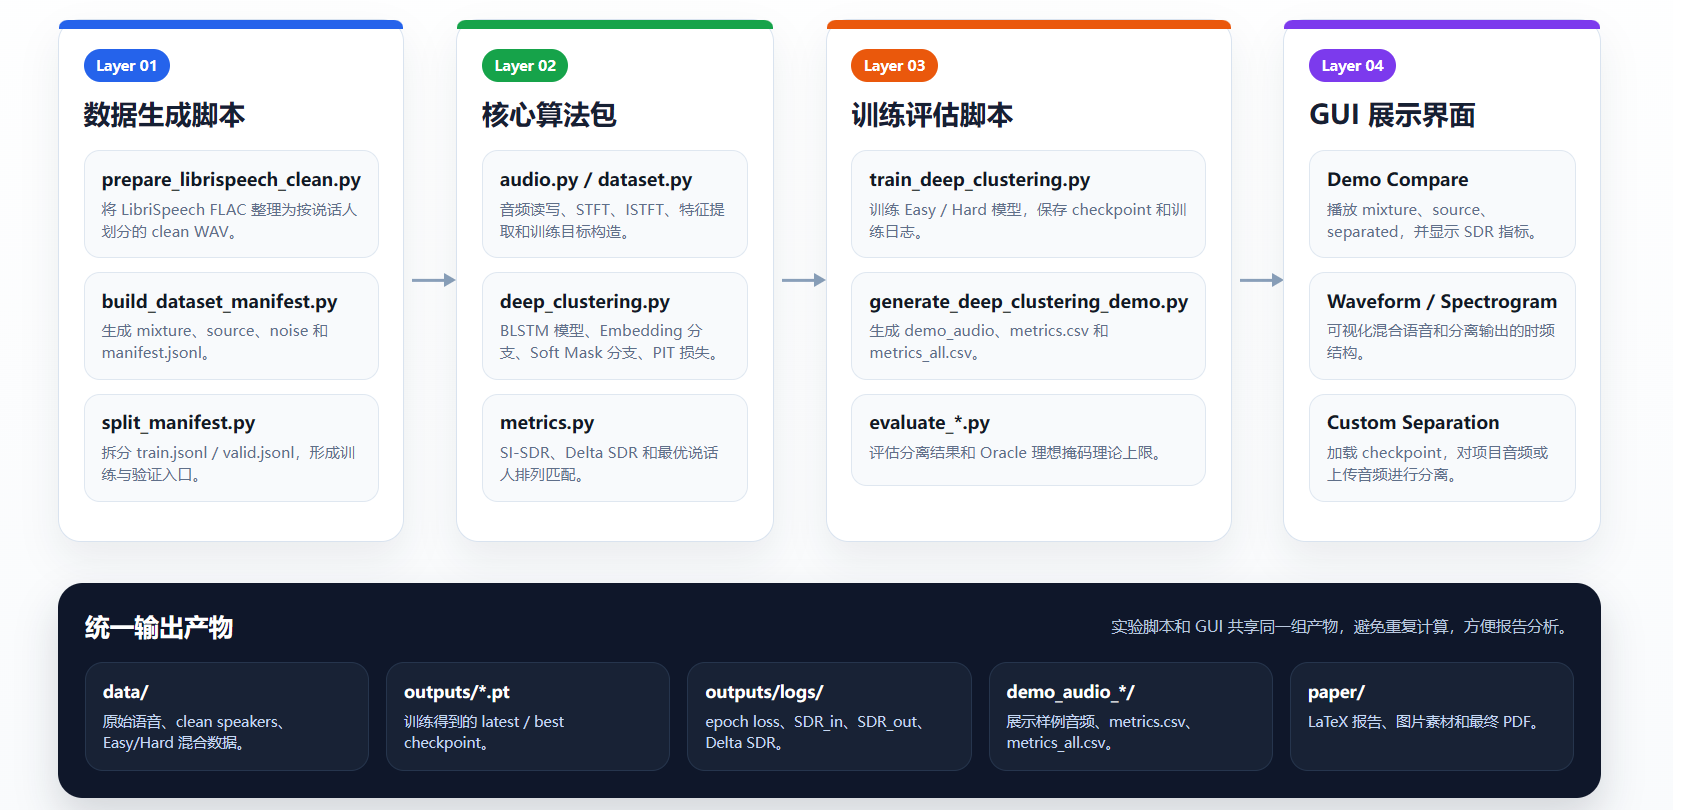
\includegraphics[width=0.95\textwidth]{code_structure.png}
    \caption{项目代码结构与数据流}
    \label{fig:code_structure}
\end{figure}

主要目录与文件功能如下：

\begin{itemize}
    \item \texttt{src/cocktail\_separation/audio.py}：负责 WAV 读写、STFT、ISTFT 和幅度归一化；
    \item \texttt{src/cocktail\_separation/dataset.py}：读取 manifest，构造训练特征、理想掩码和参考源；
    \item \texttt{src/cocktail\_separation/deep\_clustering.py}：定义 BLSTM 模型、深度聚类损失和软掩码损失；
    \item \texttt{src/cocktail\_separation/metrics.py}：实现 SI-SDR 和最优排列匹配；
    \item \texttt{src/train\_deep\_clustering.py}：训练模型并保存 checkpoint 与训练日志；
    \item \texttt{src/generate\_deep\_clustering\_demo.py}：生成 demo 音频和评估指标；
    \item \texttt{gui\_app.py}：提供音频播放、频谱展示、自定义分离和指标总览界面。
\end{itemize}

\section{模型方法与实现}

\subsection{时频特征提取}

语音分离通常在时频域中进行。实验使用短时傅里叶变换（STFT）将一维语音波形转换为复数谱：

\[
X(t, f) = \mathrm{STFT}(x)
\]

其中 $t$ 表示时间帧，$f$ 表示频率 bin。模型输入使用混合语音幅度谱的对数特征：

\[
F(t, f) = \log(1 + |X(t, f)|)
\]

随后对特征做均值方差标准化，减少不同样本音量差异对训练的影响。模型输出每个说话人的时频掩码 $M_k(t,f)$，再与混合谱相乘得到估计的说话人谱：

\[
\hat{S}_k(t,f) = M_k(t,f)X(t,f)
\]

最后通过 ISTFT 将估计谱还原为波形。

\subsection{BLSTM 软掩码模型}

模型主体位于 \texttt{src/cocktail\_separation/deep\_clustering.py}。网络结构采用 BLSTM 作为时序建模模块。BLSTM 能同时利用当前帧前后的上下文信息，对语音这种强时序相关信号更合适。

深度聚类思想最早通过学习时频单元的判别式嵌入来完成说话人分离 \cite{hershey2016deep}。本实验在该思路基础上保留 embedding 分支，同时使用更直接的软掩码分支完成语音重建。模型包含两个输出分支：

\begin{itemize}
    \item \textbf{Embedding 分支}：输出每个时频单元的嵌入向量，可用于深度聚类损失；
    \item \textbf{Mask 分支}：输出两个说话人的软掩码，直接用于语音分离。
\end{itemize}

当前主实验采用 mask 分支训练，设置 \texttt{dc-loss-weight=0.0}、\texttt{mask-loss-weight=1.0}。这样训练目标直接对齐分离后的幅度谱，更容易稳定提升 SI-SDR。

\subsection{置换不变训练损失}

语音分离存在输出顺序不确定问题：模型的第 1 路输出并不一定对应参考源 1。因此训练时使用置换不变训练\cite{yu2017pit}。对两说话人任务，计算两种输出-参考源匹配方式下的损失，并选择较小者作为当前样本损失：

\[
\mathcal{L} = \min_{\pi \in \mathcal{P}}
\sum_{k=1}^{K}
\left\|
M_k \odot |X| - |S_{\pi(k)}|
\right\|_2^2
\]

其中 $\mathcal{P}$ 表示所有说话人排列，$K=2$。该损失避免了人为固定输出顺序导致的训练冲突。

\subsection{关键代码实现}

数据生成阶段的核心是将两个参考源按比例混合，并在 Hard 实验中按指定 SNR 加入真实环境噪声。关键代码如代码 \ref{code:mix_noise} 所示。

\begin{lstlisting}[language=Python, caption={混合语音和噪声加入逻辑}, label={code:mix_noise}]
source_contribs = np.stack(
    [args.source1_gain * sources[0], args.source2_gain * sources[1]],
    axis=0,
)
mono_mix, speech_scale = peak_normalize_with_scale(
    np.sum(source_contribs, axis=0)
)
source_contribs = source_contribs * speech_scale

if noise_files:
    noise_path = Path(rng.choice(noise_files))
    noise, noise_sr = read_wav_mono(noise_path)
    noise = resample_linear(noise, noise_sr, args.sample_rate)
    mono_mix, noisy_scale = peak_normalize_with_scale(
        add_noise_at_snr(mono_mix, noise, args.snr_db, rng)
    )
    source_contribs = source_contribs * noisy_scale
\end{lstlisting}

模型使用 BLSTM 提取时序上下文，并通过 mask 分支输出两个说话人的时频掩码。代码 \ref{code:model} 展示了模型前向传播的关键部分。

\begin{lstlisting}[language=Python, caption={BLSTM 软掩码模型前向传播}, label={code:model}]
out, _ = self.blstm(features)
emb = self.proj(out).reshape(
    batch, frames * self.freq_bins, self.embedding_dim
)
emb = F.normalize(emb, p=2, dim=-1)

mask_logits = self.mask_proj(out).reshape(
    batch, frames, self.freq_bins, self.num_speakers
)
mask_logits = mask_logits.permute(0, 3, 1, 2)
masks = torch.sigmoid(mask_logits)
\end{lstlisting}

训练循环中，模型预测掩码后计算置换不变的信号逼近损失，并用 Adam 更新参数。关键代码如代码 \ref{code:train_loop} 所示。

\begin{lstlisting}[language=Python, caption={训练循环中的损失计算与参数更新}, label={code:train_loop}]
optimizer.zero_grad()
embeddings, predicted_masks = model(features, return_masks=True)
mi_loss = mask_inference_loss(
    predicted_masks, mix_magnitude, source_magnitudes, weights
)
loss = args.dc_loss_weight * dc_loss + args.mask_loss_weight * mi_loss
loss.backward()
torch.nn.utils.clip_grad_norm_(model.parameters(), max_norm=5.0)
optimizer.step()
\end{lstlisting}

\subsection{评估指标}

实验使用 SI-SDR 衡量分离质量。SI-SDR 在语音分离评估中常用于减少整体缩放差异对指标的影响 \cite{leroux2019sdr}。对估计语音 $\hat{s}$ 和参考语音 $s$，先将估计语音投影到参考语音方向：

\[
s_{\mathrm{target}} = \frac{\langle \hat{s}, s\rangle}{\|s\|^2}s
\]

再计算目标成分与误差成分的能量比：

\[
\mathrm{SI\mbox{-}SDR}
= 10\log_{10}
\frac{\|s_{\mathrm{target}}\|^2}
{\|\hat{s}-s_{\mathrm{target}}\|^2}
\]

报告中主要使用三个指标：

\begin{itemize}
    \item \textbf{SDR\_in}：分离前混合语音相对参考源的 SI-SDR；
    \item \textbf{SDR\_out}：分离后输出语音相对参考源的 SI-SDR；
    \item \textbf{Delta\_SDR}：$SDR\_out - SDR\_in$，表示分离带来的改善幅度。
\end{itemize}

评估时同样考虑说话人排列问题，脚本会枚举所有输出和参考源的匹配方式，取平均 SI-SDR 最高的排列作为最终结果。

\section{实验结果与评估}

\subsection{训练设置与日志分析}

Easy 和 Hard 模型均使用 \texttt{train\_deep\_clustering.py} 训练。主要参数保持一致：

\begin{itemize}
    \item 训练轮数：200 epochs；
    \item batch size：4；
    \item 优化器：Adam；
    \item 学习率：$1\times 10^{-3}$；
    \item BLSTM hidden size：300；
    \item LSTM 层数：2；
    \item STFT 参数：\texttt{n\_fft=512}，\texttt{hop\_length=128}；
    \item 损失权重：\texttt{dc-loss-weight=0.0}，\texttt{mask-loss-weight=1.0}。
\end{itemize}

Easy 日志文件为 \texttt{deep\_clustering\_easy\_20260606\_144753.csv}，验证集最佳记录出现在第 100 个 epoch：\texttt{SDR\_in=-0.013 dB}，\texttt{SDR\_out=6.953 dB}，\texttt{Delta\_SDR=6.966 dB}。

Hard 日志文件为 \texttt{deep\_clustering\_hard\_20260604\_214512.csv}，验证集最佳记录出现在第 165 个 epoch：\texttt{SDR\_in=-0.933 dB}，\texttt{SDR\_out=1.617 dB}，\texttt{Delta\_SDR=2.549 dB}。

图 \ref{fig:results_training_curves} 展示了 Easy 与 Hard 的训练 loss 和验证指标变化。两组实验的训练 loss 都随 epoch 增加而下降，说明模型能够逐步拟合训练样本。Easy 验证集指标整体高于 Hard，说明在无噪声、说话人池较小、混合比例不完全均衡的条件下，模型更容易学习稳定的分离规律。Hard 验证集受真实环境噪声、说话人数量增加和 0.5:0.5 强重叠影响，验证指标提升更困难。

\begin{figure}[H]
    \centering
    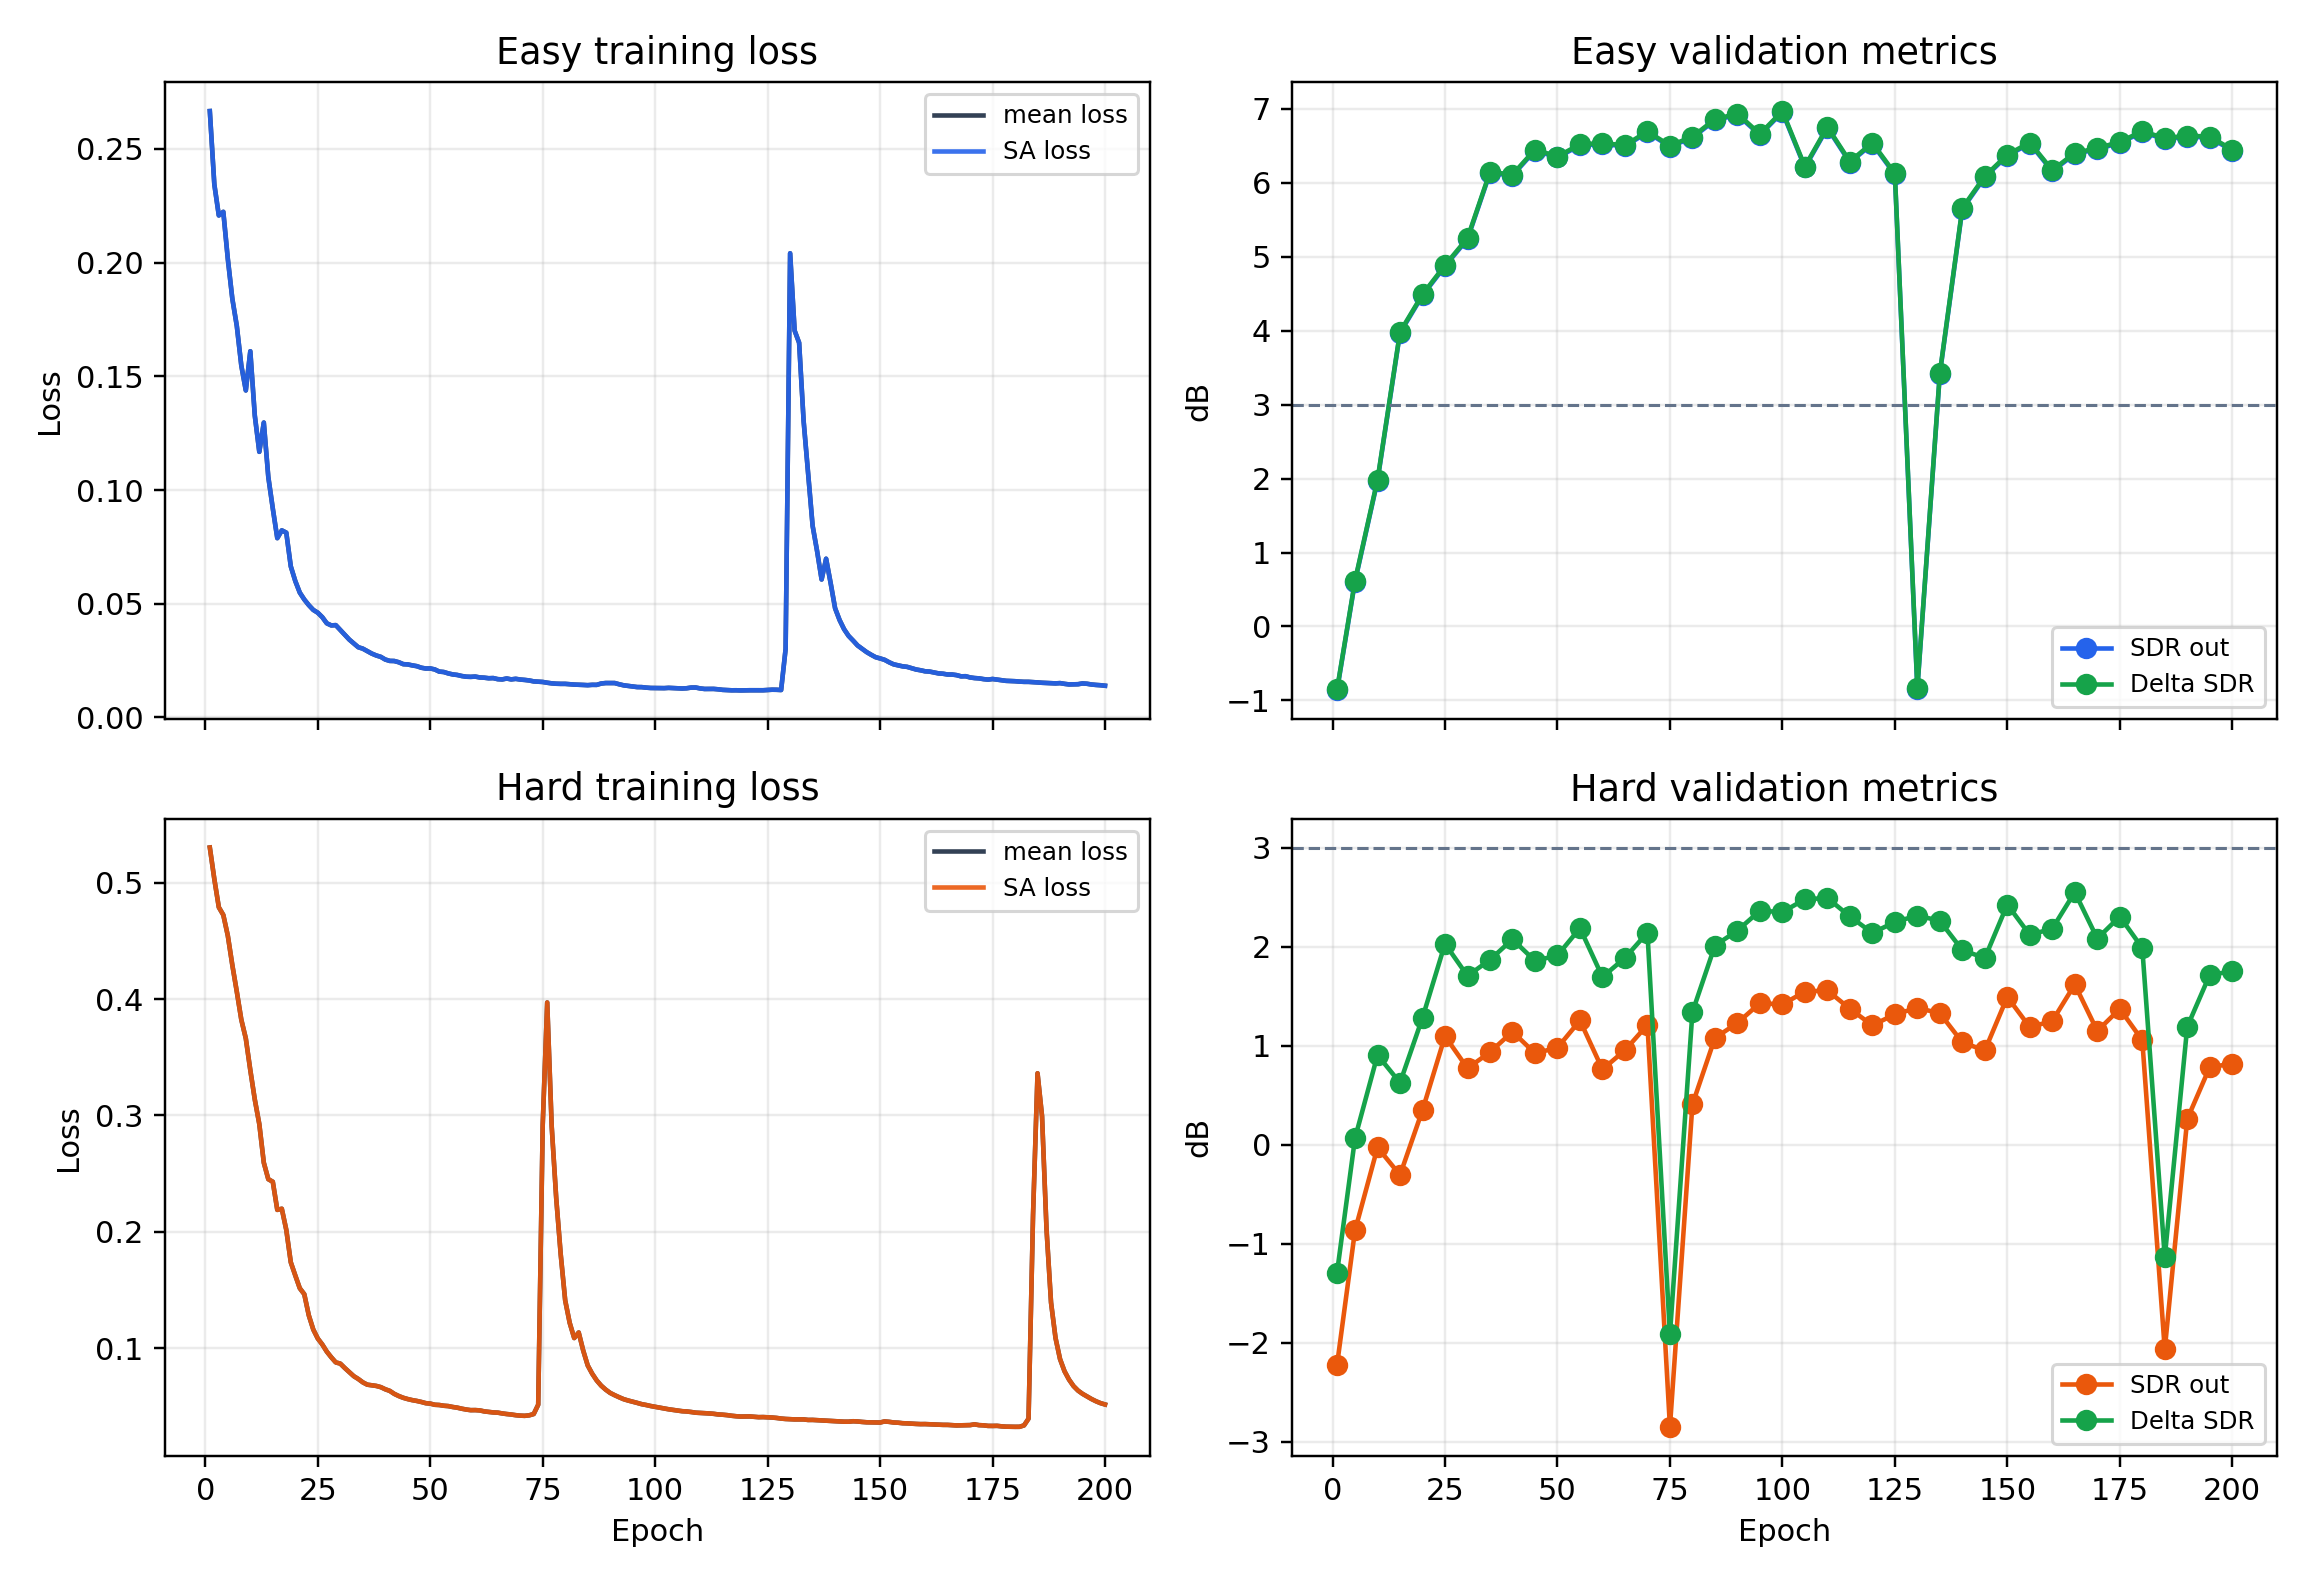
\includegraphics[width=0.95\textwidth]{results_training_curves_easy_hard.png}
    \caption{Easy 与 Hard 模型训练 loss 和验证 SI-SDR 曲线}
    \label{fig:results_training_curves}
\end{figure}

\subsection{整体评估结果}

表 \ref{tab:metrics_summary} 和图 \ref{fig:metrics_summary} 汇总了 Easy 与 Hard 两组实验在验证集和精选展示样例上的指标。其中 selected 表示从验证集中选择的 3 个展示样例，valid all 表示完整验证集平均结果。

\begin{table}[H]
    \centering
    \caption{Easy 与 Hard 实验 SI-SDR 结果}
    \label{tab:metrics_summary}
    \begin{tabular}{lccc}
        \toprule
        数据范围 & SDR\_in / dB & SDR\_out / dB & Delta\_SDR / dB \\
        \midrule
        Easy selected & -0.022 & 12.803 & 12.825 \\
        Easy valid all & -0.013 & 6.953 & 6.966 \\
        Hard selected & -0.884 & 9.835 & 10.719 \\
        Hard valid all & -0.933 & 1.617 & 2.549 \\
        \bottomrule
    \end{tabular}
\end{table}

\begin{figure}[H]
    \centering
    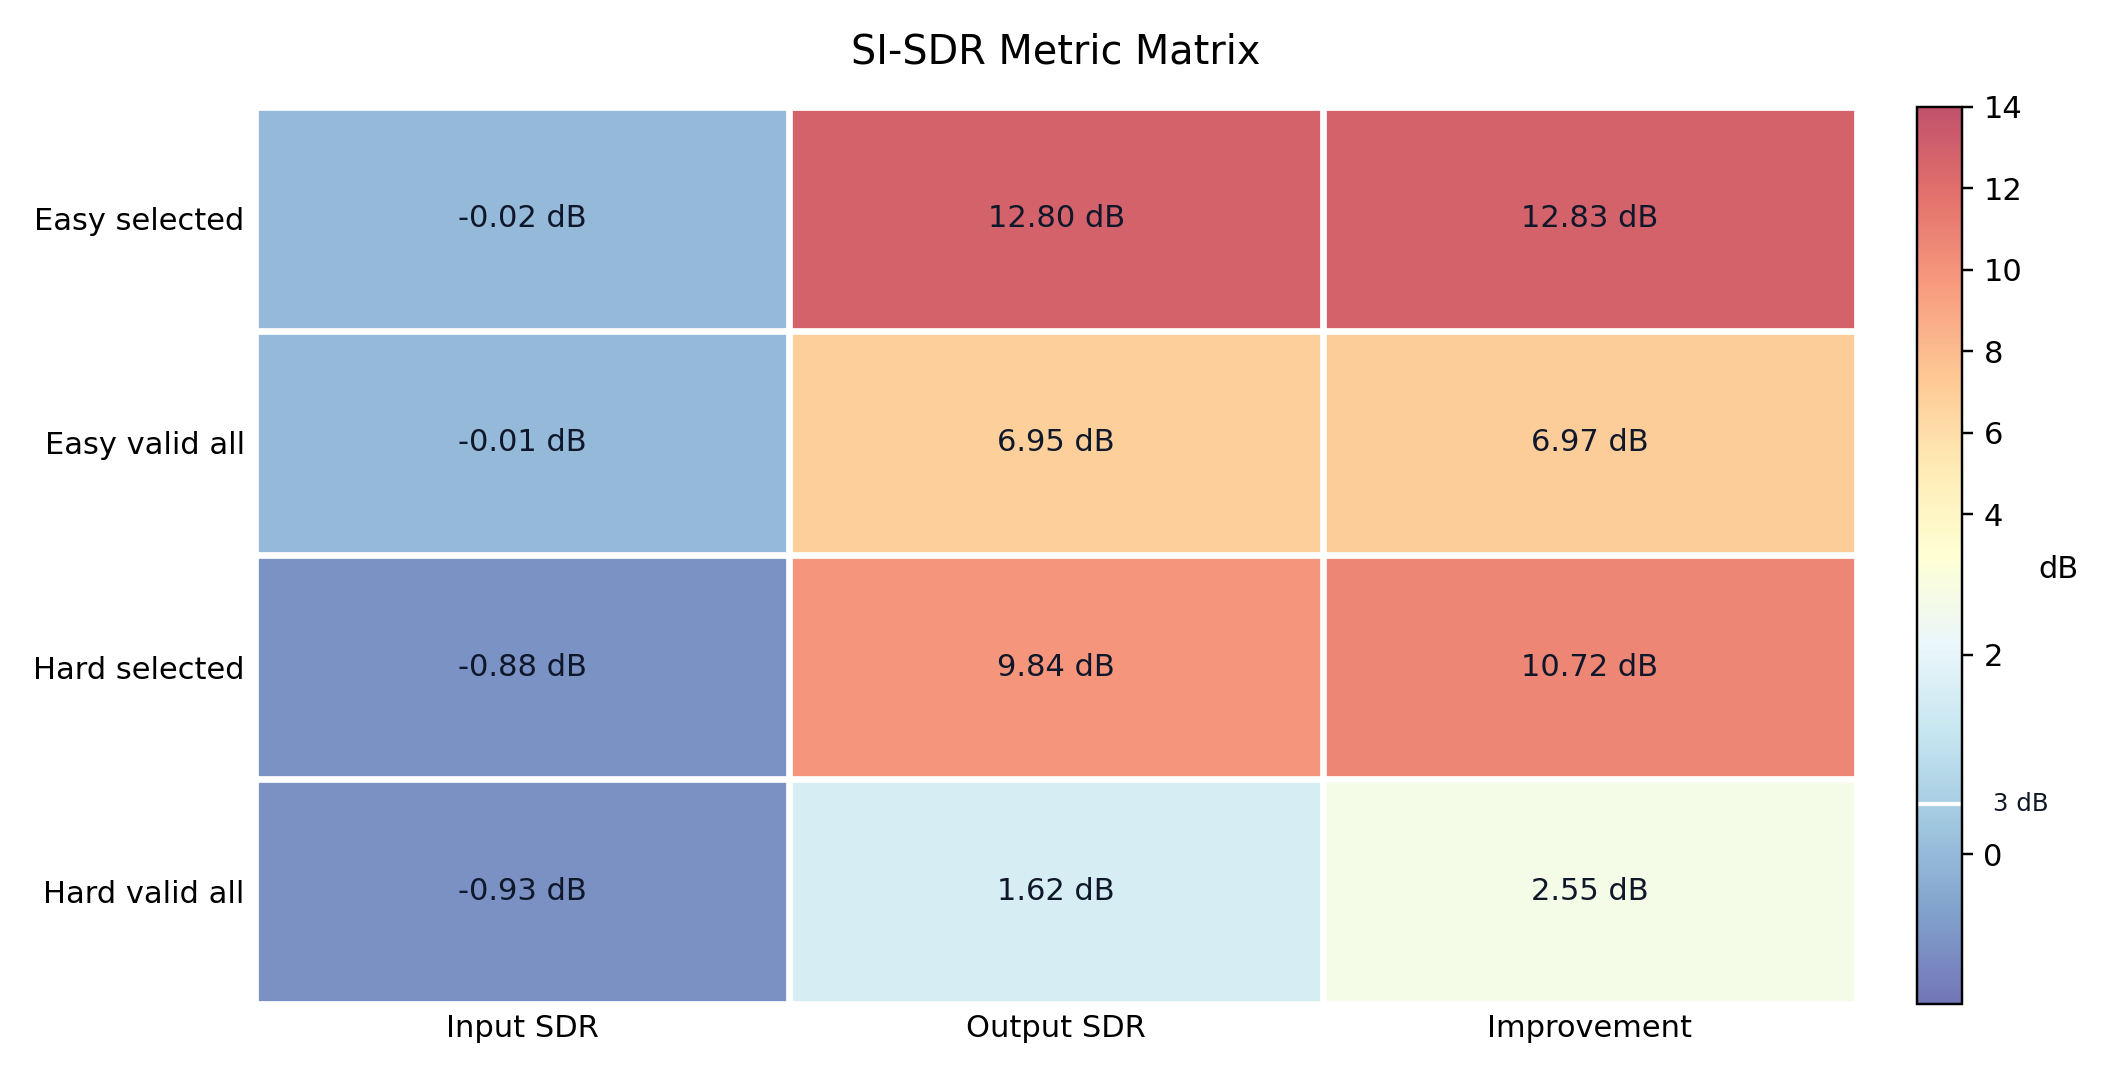
\includegraphics[width=0.92\textwidth]{results_metrics_summary.png}
    \caption{Easy 与 Hard 验证集和展示样例 SI-SDR 指标热力矩阵}
    \label{fig:metrics_summary}
\end{figure}

从完整验证集平均结果看，Easy 实验的 \texttt{Delta\_SDR=6.966 dB}，明显超过 3 dB 改善标准，说明模型在简单双说话人混合条件下能够有效提升语音质量。Hard 实验完整验证集的 \texttt{Delta\_SDR=2.549 dB}，略低于 3 dB，但仍相比分离前有正向改善。该下降符合预期，因为 Hard 同时增加了说话人数、提高了两人语音能量重叠程度，并加入 ESC-50 真实环境噪声。

\subsection{展示样例结果}

为了在报告和 GUI 中直观展示分离效果，实验从验证集中选择 \texttt{SDR\_out} 较高的样例生成 demo 音频。Easy 的三个展示样例均达到约 13 dB 的 \texttt{SDR\_out}；Hard 的展示样例虽然来自困难条件，但最优样例也能达到 10 dB 以上的 \texttt{SDR\_out}。

以 Easy 的第 1 个展示样例为例，分离前混合语音 \texttt{SDR\_in=0.060 dB}，分离后 \texttt{SDR\_out=13.701 dB}，提升 \texttt{13.640 dB}。图 \ref{fig:audio_vis} 展示了混合语音和两路分离语音的波形与频谱。分离结果在时频结构上更接近单一说话人，频谱重叠区域被模型分配到不同输出通道中。

\begin{figure}[H]
    \centering
    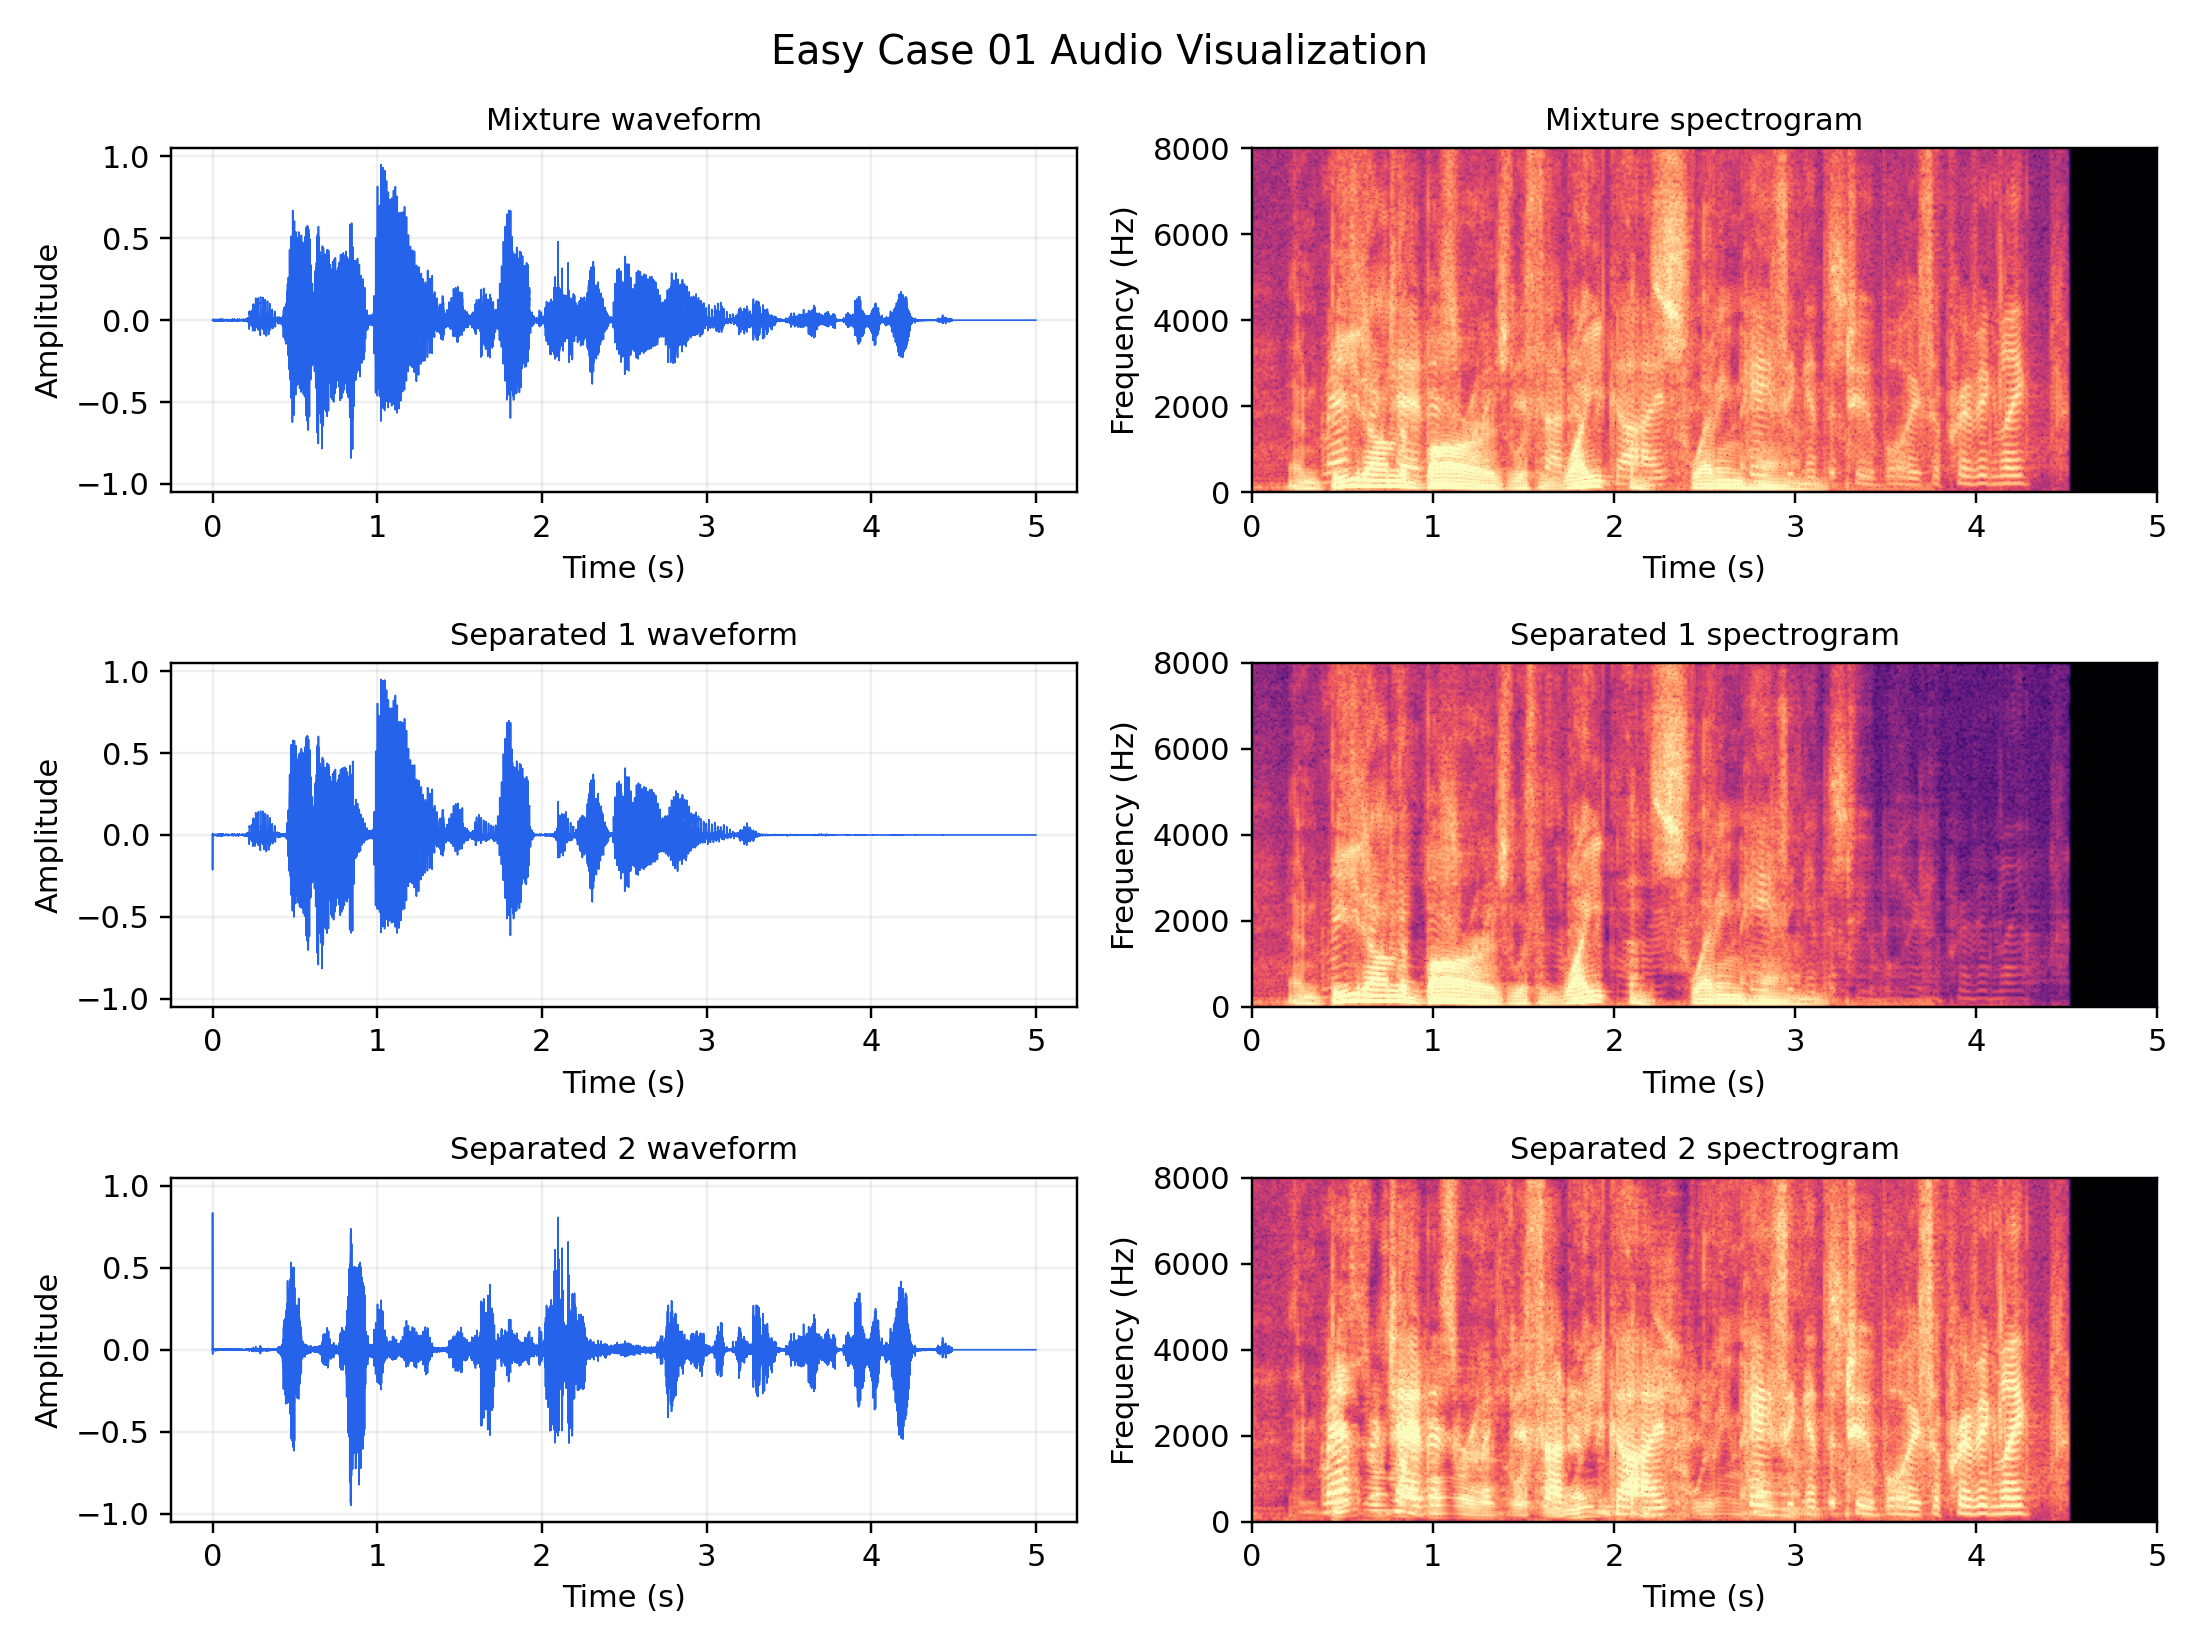
\includegraphics[width=0.95\textwidth]{results_easy_case_visualization.png}
    \caption{Easy case 01 的波形与频谱可视化}
    \label{fig:audio_vis}
\end{figure}

Hard 的第 1 个展示样例是 Hard 验证集中分离效果较好的样本，分离前 \texttt{SDR\_in=-0.666 dB}，分离后 \texttt{SDR\_out=10.624 dB}，提升 \texttt{11.290 dB}。图 \ref{fig:hard_audio_vis} 展示了该样例的波形与频谱。可以看到，虽然 Hard 场景包含真实环境噪声和更强语音重叠，但在部分验证样本上模型仍能得到较清晰的两路输出。

\begin{figure}[H]
    \centering
    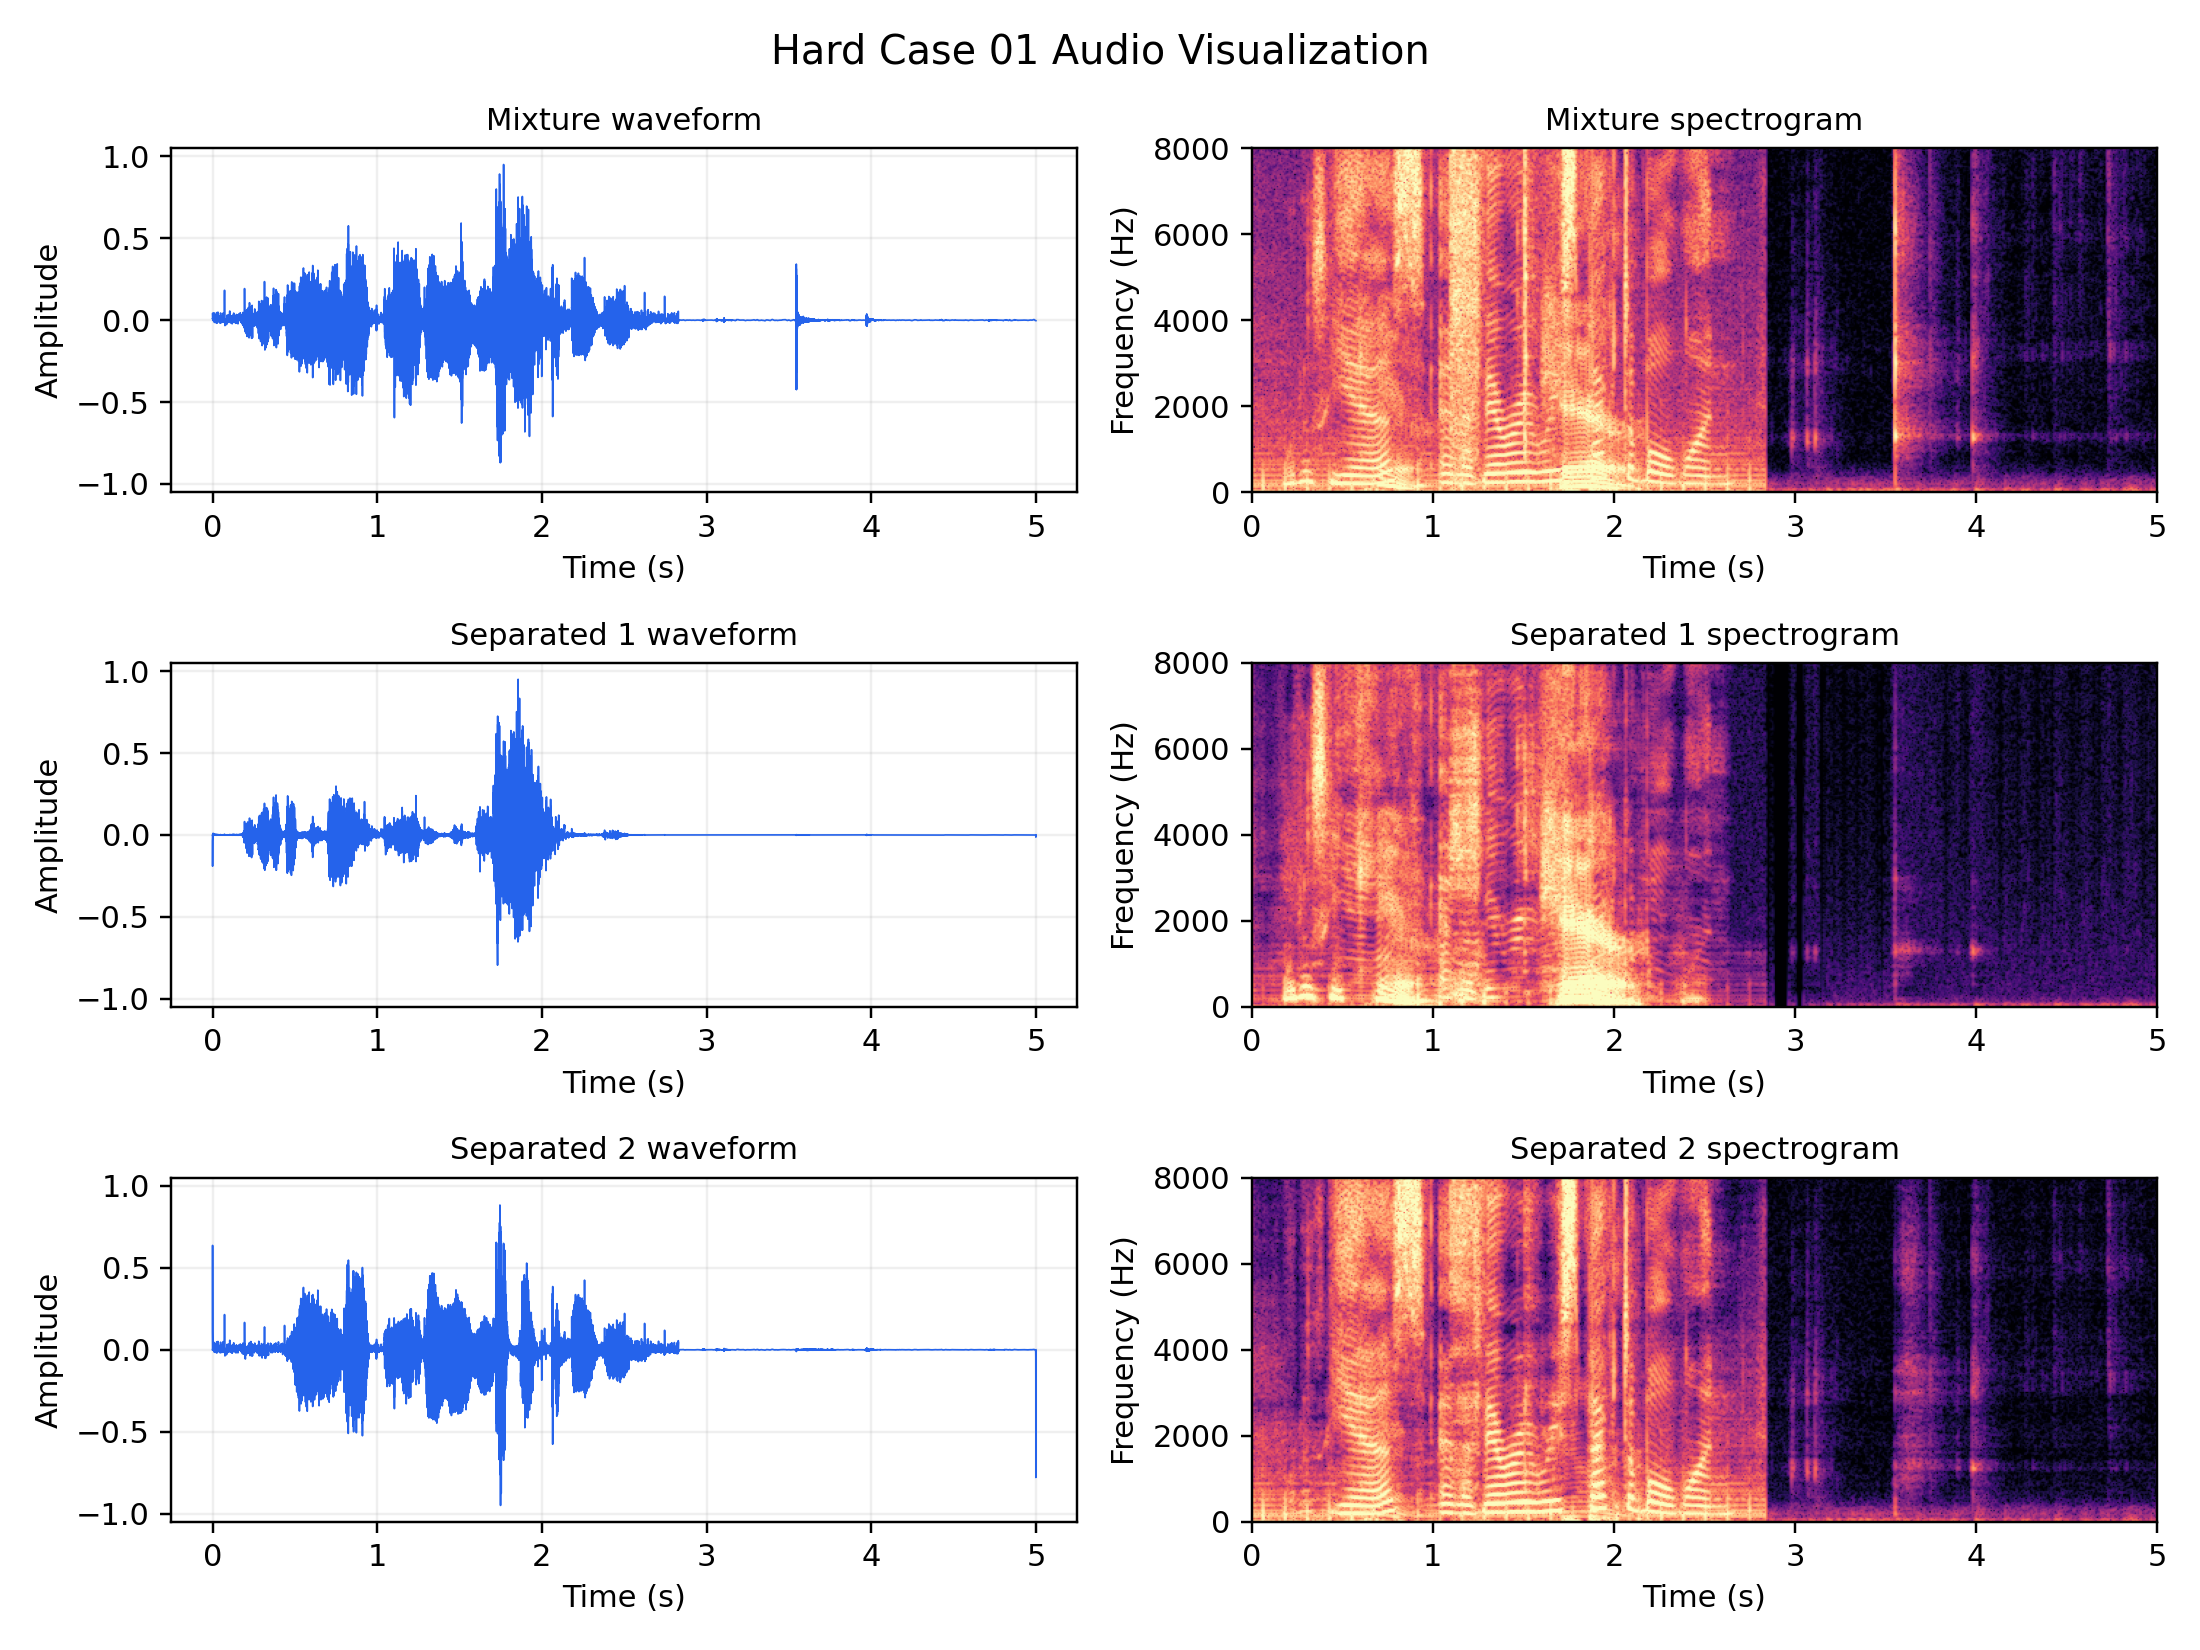
\includegraphics[width=0.95\textwidth]{results_hard_case_visualization.png}
    \caption{Hard case 01 的波形与频谱可视化}
    \label{fig:hard_audio_vis}
\end{figure}

\subsection{训练集与验证集泛化对比}

除验证集和展示样例外，本实验还分别评估了 Easy 和 Hard 模型在训练集与验证集上的表现，结果如表 \ref{tab:train_valid} 和图 \ref{fig:train_valid} 所示。

\begin{table}[H]
    \centering
    \caption{训练集与验证集平均指标对比}
    \label{tab:train_valid}
    \begin{tabular}{lccc}
        \toprule
        数据范围 & SDR\_in / dB & SDR\_out / dB & Delta\_SDR / dB \\
        \midrule
        Easy train & 0.012 & 11.064 & 11.053 \\
        Easy valid & -0.013 & 6.953 & 6.966 \\
        Hard train & -0.946 & 7.271 & 8.217 \\
        Hard valid & -0.933 & 1.617 & 2.549 \\
        \bottomrule
    \end{tabular}
\end{table}

\begin{figure}[H]
    \centering
    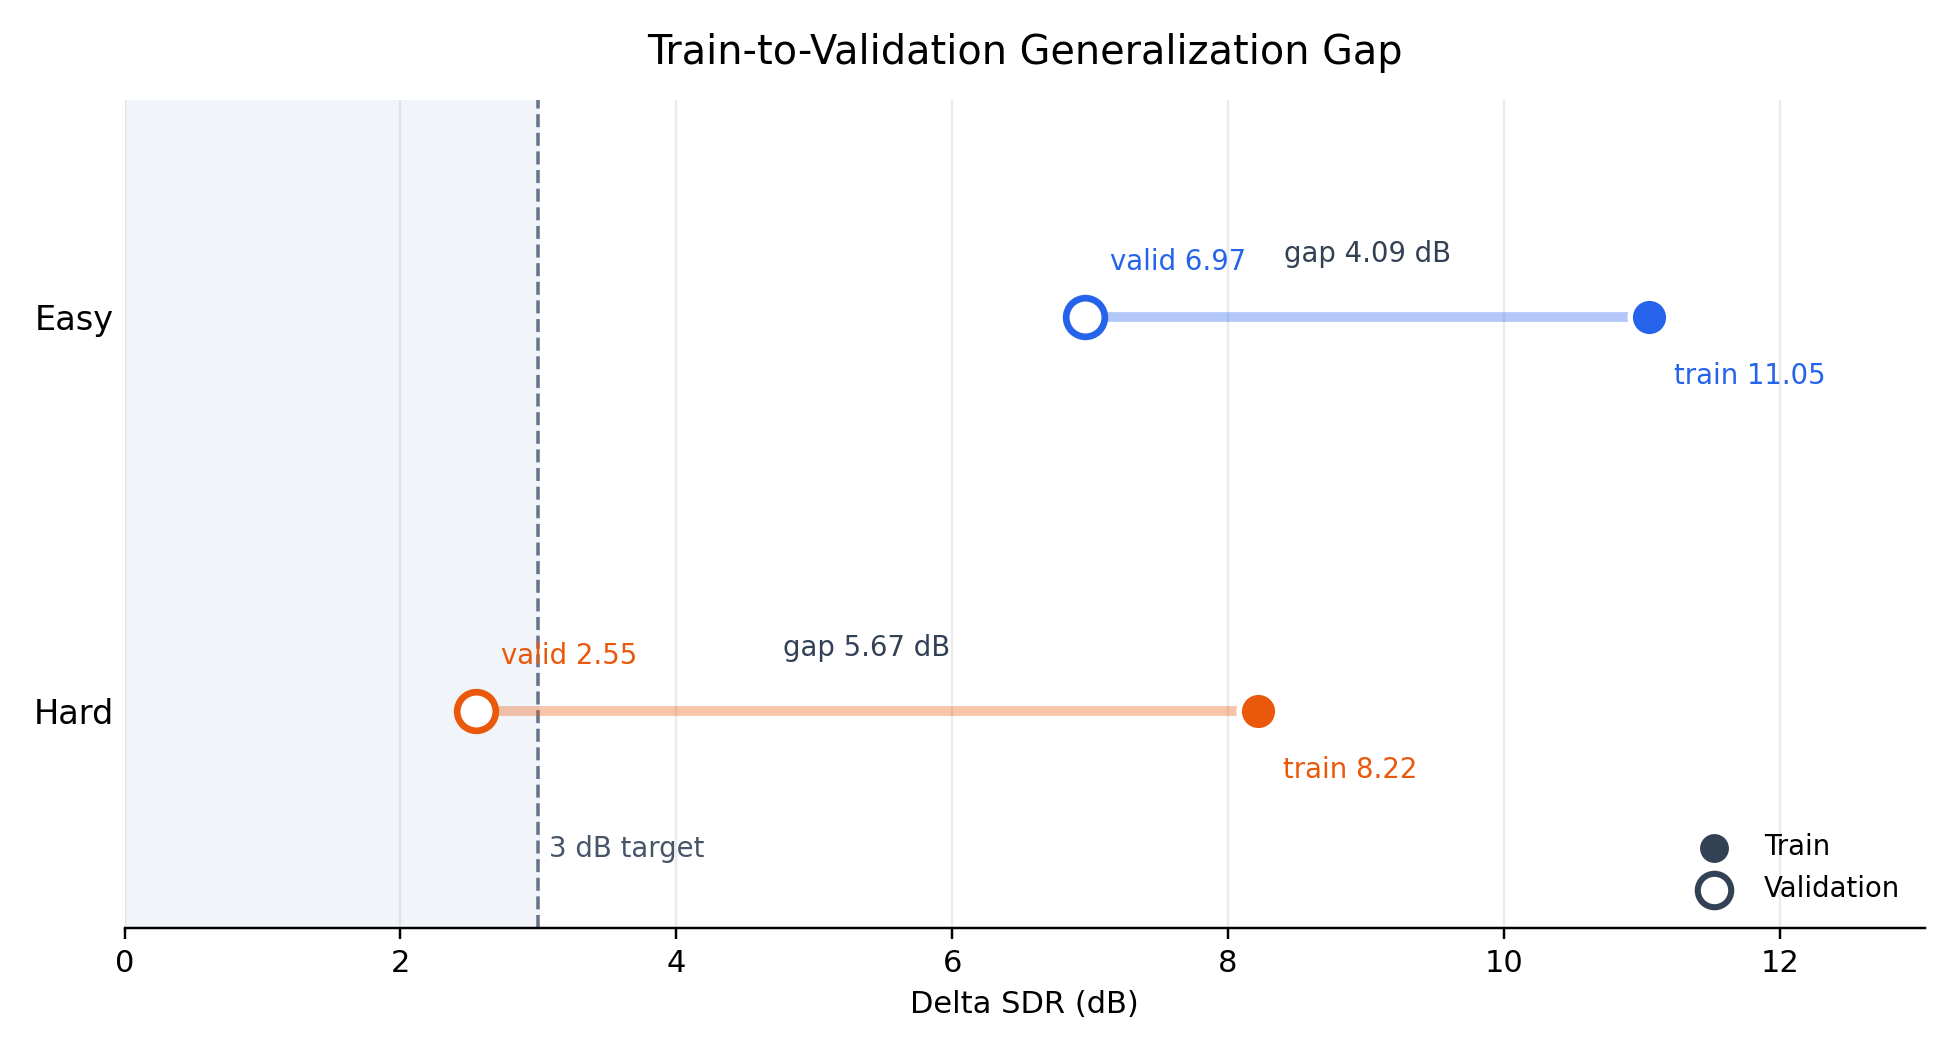
\includegraphics[width=0.88\textwidth]{results_train_valid_comparison.png}
    \caption{Easy 与 Hard 模型从训练集到验证集的 Delta SDR 泛化落差}
    \label{fig:train_valid}
\end{figure}

可以看到，Easy 和 Hard 模型在训练集上的效果都明显优于验证集。Easy 训练集平均 \texttt{Delta\_SDR=11.053 dB}，验证集下降到 \texttt{6.966 dB}；Hard 训练集平均 \texttt{Delta\_SDR=8.217 dB}，验证集下降到 \texttt{2.549 dB}。这说明当前模型已经学到了训练样本中的分离规律，但泛化能力仍然有限，尤其在 Hard 条件下表现更明显。

这一现象需要客观承认。当前模型训练受到个人设备、训练时间和数据规模限制：训练样本数量不大，Hard 数据又同时包含更多说话人、更强重叠和真实噪声，因此验证集上出现性能下降是合理的。另一方面，程序中提供的 Oracle 理想掩码评估说明，该任务在数据层面的理论上限仍然较高。例如 Easy 验证集的 Oracle \texttt{SDR\_out} 约为 \texttt{12.783 dB}，\texttt{Delta\_SDR} 约为 \texttt{12.796 dB}，说明如果掩码预测足够准确，模型仍有较大提升空间。

\subsection{失败案例与改进反思}

本实验在最终形成 Easy 和 Hard 两组结果之前，也经历过若干效果不理想的早期尝试。由于这些尝试发生在实验初期，当时没有完整保留训练日志和音频样例，因此本节主要从实验过程记录和后续改进结果出发进行反思。

第一个失败案例是训练轮数设置过少。实验最初只设置了 50 个 epoch，模型在训练尚未充分收敛时就提前结束。对于双说话人语音分离任务，模型不仅需要学习语音与噪声、说话人与说话人之间的时频差异，还需要在输出通道之间形成稳定的分配关系。如果训练轮数不足，loss 虽然可能已经开始下降，但验证集上的 \texttt{SDR\_out} 和 \texttt{Delta\_SDR} 往往还没有进入较稳定的阶段。后续将训练轮数扩大到 200 个 epoch 后，Easy 模型的最佳验证结果出现在第 100 个 epoch，Hard 模型的最佳验证结果出现在第 165 个 epoch，这说明早期 50 个 epoch 的设置确实不足以观察模型的较优状态。

第二个失败案例是训练音频数量过少。实验最初采用约 \texttt{train40+valid10} 的小规模划分，训练样本覆盖的说话人组合、混合比例和语音内容都很有限，导致模型很容易只记住少量训练样本中的局部规律，而难以学习更通用的分离特征。在这种设置下，即使继续增加训练轮数，模型能够从数据中获得的新信息也很少，验证集指标提升不明显。后续扩大训练和验证样本规模后，模型在 Easy 条件下能够获得更稳定的 SI-SDR 改善，Hard 条件下也能在部分样本上产生较清晰的分离结果。

第三个失败经验是早期缺少理论上限检查和过拟合检查。最初只关注模型输出音频是否“听起来有所分离”，没有同步计算 Oracle 理想掩码结果，也没有比较训练集与验证集上的指标差异。因此，如果算法实现、数据生成或评估流程中存在问题，很难判断是任务本身过难、模型能力不足，还是程序环节存在错误。后续加入 Oracle 评估后，可以确认数据层面的理论上限仍然较高；加入训练集与验证集对比后，也能更清楚地看到当前模型在验证集上的泛化能力有限。这些检查使实验从单纯观察结果转向了更可解释的误差分析，也为后续改进模型结构、增加数据规模和调整训练策略提供了依据。

\subsection{最优与最差样本分析}

完整验证集评估还可以观察模型的稳定性。Easy 验证集中最优样本为 manifest index 26，\texttt{SDR\_out=13.701 dB}，\texttt{Delta\_SDR=13.640 dB}；最差样本为 manifest index 43，\texttt{Delta\_SDR=-3.598 dB}。Hard 验证集中最优样本为 manifest index 31，\texttt{SDR\_out=10.624 dB}，\texttt{Delta\_SDR=11.290 dB}；最差样本为 manifest index 16，\texttt{Delta\_SDR=-11.745 dB}。

这些失败样例说明模型仍存在泛化不足问题。原因包括：两位说话人的音色或频谱分布相近、语音重叠程度过高、环境噪声与语音频段重合、训练样本数量有限等。同时，验证集中也存在分离效果较好的样本。Easy 验证集最优样本达到 \texttt{SDR\_out=13.701 dB}，Hard 验证集最优样本达到 \texttt{SDR\_out=10.624 dB}。这些样例表明，虽然当前模型整体泛化仍有限，但在部分验证样本上已经能够产生较清晰的分离结果，说明实验流程和模型方向是有效的。

\section{GUI 设计说明}

\subsection{设计目标}

命令行脚本可以完成训练和评估，但实验展示时仅依赖终端输出不够直观。因此项目设计了基于 Streamlit 的 GUI 入口 \texttt{gui\_app.py}。GUI 的目标不是替代训练脚本，而是把已有实验结果组织成可听、可看、可比较的展示界面。

GUI 主要服务于以下场景：

\begin{itemize}
    \item 快速播放 Easy 与 Hard 的混合语音、参考源和分离结果；
    \item 对比波形和频谱，观察分离前后的时频结构变化；
    \item 选择 checkpoint 对单条混合语音或上传音频进行分离；
    \item 汇总 demo 指标、完整验证集指标和训练日志曲线。
\end{itemize}

\subsection{页面结构}

GUI 采用侧边栏导航，包含四个页面：

\begin{enumerate}
    \item \textbf{Demo Compare}：选择 Easy 或 Hard 以及具体 case，播放 \texttt{mixture.wav}、\texttt{source\_1.wav}、\texttt{source\_2.wav}、\texttt{separated\_1.wav} 和 \texttt{separated\_2.wav}，并展示 \texttt{SDR\_in}、\texttt{SDR\_out}、\texttt{Delta\_SDR} 与最优排列。
    \item \textbf{Waveform And Spectrogram}：对选中音频绘制 waveform 与 spectrogram。该页面用于解释模型如何在时频域中把混合语音拆分为两路输出。
    \item \textbf{Custom Separation}：选择 \texttt{outputs/*.pt} checkpoint 和项目中的混合 WAV，或上传新的 WAV 文件，运行模型并保存分离结果。
    \item \textbf{Metrics Overview}：读取 \texttt{metrics.csv}、\texttt{metrics\_all.csv} 和 \texttt{outputs/logs/*.csv}，显示 Easy/Hard 指标表格、柱状图和训练曲线。
\end{enumerate}

图 \ref{fig:gui_mockup} 给出了 GUI 主页面的结构示意。界面设计优先保证实验数据可读性：左侧为页面导航，主区域展示 case 选择、指标卡片和音频播放器。

\begin{figure}[H]
    \centering
    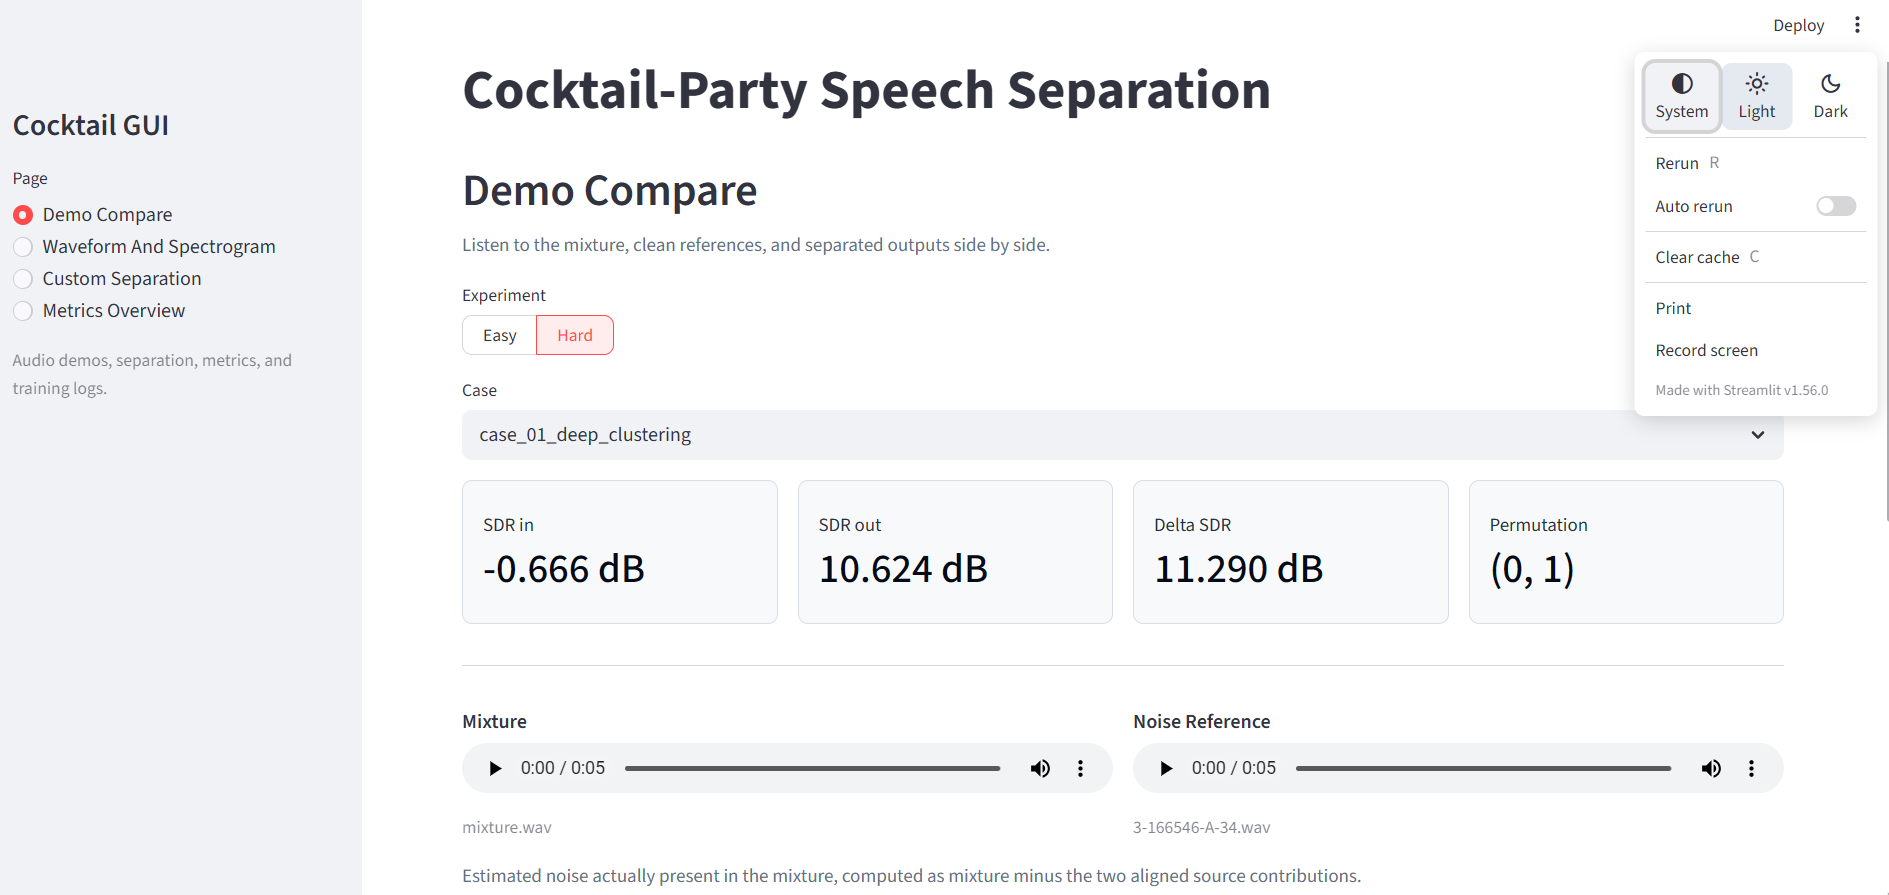
\includegraphics[width=0.9\textwidth]{gui_design_mockup.png}
    \caption{GUI 主页面结构示意}
    \label{fig:gui_mockup}
\end{figure}

\subsection{噪声展示设计}

Hard 实验中 mixture 已经加入真实环境噪声，但在 10 dB SNR 条件下，噪声可能被人声部分遮盖，主观听感不一定非常明显。因此 GUI 对 Hard 样例提供两类噪声展示：

\begin{itemize}
    \item \textbf{Noise Reference}：数据生成时使用的 ESC-50 噪声素材或 demo 目录中保存的噪声片段；
    \item \textbf{Estimated Noise In Mixture}：由 GUI 根据 \texttt{mixture - source\_1 - source\_2} 估算得到的混合语音中实际噪声成分。
\end{itemize}

第二类音频会保存到 \texttt{outputs/gui\_noise\_estimates/}。这种设计可以帮助区分“噪声素材本身”和“实际混进语音后的噪声残差”，避免展示时误以为 Hard mixture 没有加入噪声。

GUI 中估计混合语音实际噪声的核心代码如代码 \ref{code:gui_noise} 所示。该方法读取 manifest 中记录的 mixture 和 sources，并通过残差近似得到实际噪声成分。

\begin{lstlisting}[language=Python, caption={GUI 中估计 Hard mixture 实际噪声成分}, label={code:gui_noise}]
mixture, sr = read_audio(resolve_project_path(manifest_row["mixture"]))
sources = [
    read_audio(resolve_project_path(path), sr)[0]
    for path in manifest_row["sources"]
]
n = min([mixture.shape[0], *(source.shape[0] for source in sources)])
residual = mixture[:n] - np.sum(
    np.stack([source[:n] for source in sources], axis=0),
    axis=0,
)
sf.write(str(out_path), normalize_peak(residual), sr)
\end{lstlisting}

自定义分离页面复用了训练脚本保存的 checkpoint。前端选择 checkpoint 和 mixture 后，程序加载模型、计算 STFT、预测掩码并写出两路分离音频，关键流程如代码 \ref{code:gui_separate} 所示。

\begin{lstlisting}[language=Python, caption={GUI 自定义音频分离流程}, label={code:gui_separate}]
torch, model, ckpt, device, num_speakers = load_model(
    str(checkpoint), device_preference
)
mixture, sample_rate = read_audio(mixture_path)
spec = stft(mixture, n_fft=int(ckpt["n_fft"]),
            hop_length=int(ckpt["hop_length"]))
features = np.log1p(np.abs(spec).astype(np.float32))[None, :, :]

with torch.no_grad():
    x = torch.as_tensor(features, dtype=torch.float32, device=device)
    _, predicted_masks = model(x, return_masks=True)
    masks = predicted_masks[0].detach().cpu().numpy()
\end{lstlisting}

\subsection{输出目录}

GUI 保持与原实验脚本相同的数据组织方式，不改变已有训练和评估脚本。自定义上传音频保存到：

\begin{center}
\texttt{outputs/gui\_uploads/}
\end{center}

GUI 分离结果保存到：

\begin{center}
\texttt{outputs/gui\_separated/}
\end{center}

这种目录设计可以避免覆盖原有 demo 音频和训练输出，同时便于后续查看 GUI 交互产生的新结果。

\section{总结与改进方向}

本实验完成了一个较完整的鸡尾酒会语音分离系统。数据层面，实验从 LibriSpeech 中整理真实说话人语音，构造 Easy 和 Hard 两组双说话人混合数据，并在 Hard 实验中加入 ESC-50 真实环境噪声。模型层面，实验采用 STFT 特征、BLSTM 时序建模、软掩码预测和 PIT 损失，实现了从混合语音到两路分离语音的端到端处理流程。评估层面，实验使用 SI-SDR、Delta SDR 和最优排列匹配衡量分离效果。

实验结果表明，模型在 Easy 验证集上取得了明显改善，完整验证集平均 \texttt{Delta\_SDR=6.966 dB}，精选展示样例的 \texttt{SDR\_out} 可达到 13 dB 以上，主观听感较清晰。Hard 实验由于引入更复杂说话人池、等能量混合和真实环境噪声，完整验证集平均 \texttt{Delta\_SDR=2.549 dB}，低于 Easy，但最佳展示样例仍能达到 10 dB 以上的 \texttt{SDR\_out}。这说明模型具备基础分离能力，但在噪声和强重叠条件下仍有提升空间。

同时，训练集与验证集对比显示，Easy 和 Hard 模型的验证效果都没有训练集效果好，说明当前模型的泛化能力有限。这一点与个人设备、训练时间和数据规模限制有关：在有限样本上训练 200 个 epoch 能够让模型较好拟合训练集，但在未见过的说话人与噪声组合上仍容易下降。不过，从 Oracle 理想掩码结果以及部分验证样例的高质量分离效果可以看出，数据和程序流程本身具有较高理论上限，后续通过扩大数据、延长训练、改进模型结构仍有继续提升空间。

GUI 部分将命令行实验结果转化为可交互展示系统，支持 demo 播放、波形与频谱可视化、自定义音频分离和指标总览。它使实验结果不再只停留在 CSV 和终端输出中，而是可以通过听觉和视觉方式直接验证分离效果。

后续改进方向包括：

\begin{enumerate}
    \item \textbf{扩大训练数据规模}：当前训练样本数量较小，模型对复杂说话人和噪声场景的泛化能力有限。增加更多说话人、更多语音片段和更多噪声类型有助于提升稳定性。
    \item \textbf{改进模型结构}：可以尝试 Conv-TasNet、Dual-Path RNN、SepFormer 等更强的语音分离模型，减少手工 STFT 特征依赖并提升端到端建模能力。
    \item \textbf{增强噪声鲁棒性}：Hard 实验中噪声显著影响分离质量，后续可加入不同 SNR 的噪声增强、混响增强或多条件训练。
    \item \textbf{完善 GUI 功能}：可继续加入批量分离、失败案例筛选、指标排序、音频下载按钮和模型对比页面，使 GUI 更接近完整实验分析平台。
    \item \textbf{补充主观评价}：除 SI-SDR 外，可以加入 PESQ、STOI 或人工听感评价，更全面地衡量分离语音的可懂度和自然度。
\end{enumerate}

总体而言，本实验实现了从数据生成、模型训练、结果评估到 GUI 展示的完整流程，能够较好地说明基础盲语音分离方法在简单和困难条件下的表现差异。


\begin{thebibliography}{9}

\bibitem{panayotov2015librispeech}
V. Panayotov, G. Chen, D. Povey, and S. Khudanpur.
\newblock Librispeech: An ASR corpus based on public domain audio books.
\newblock In \emph{Proceedings of the IEEE International Conference on Acoustics, Speech and Signal Processing (ICASSP)}, pp. 5206--5210, 2015.

\bibitem{piczak2015esc}
K. J. Piczak.
\newblock ESC: Dataset for environmental sound classification.
\newblock In \emph{Proceedings of the 23rd ACM International Conference on Multimedia}, pp. 1015--1018, 2015.

\bibitem{hershey2016deep}
J. R. Hershey, Z. Chen, J. Le Roux, and S. Watanabe.
\newblock Deep clustering: Discriminative embeddings for segmentation and separation.
\newblock In \emph{Proceedings of the IEEE International Conference on Acoustics, Speech and Signal Processing (ICASSP)}, pp. 31--35, 2016.

\bibitem{yu2017pit}
D. Yu, M. Kolb{\ae}k, Z.-H. Tan, and J. Jensen.
\newblock Permutation invariant training of deep models for speaker-independent multi-talker speech separation.
\newblock In \emph{Proceedings of the IEEE International Conference on Acoustics, Speech and Signal Processing (ICASSP)}, pp. 241--245, 2017.

\bibitem{leroux2019sdr}
J. Le Roux, S. Wisdom, H. Erdogan, and J. R. Hershey.
\newblock SDR -- half-baked or well done?
\newblock In \emph{Proceedings of the IEEE International Conference on Acoustics, Speech and Signal Processing (ICASSP)}, pp. 626--630, 2019.

\end{thebibliography}

\end{document}
